\chapter{Materiais e Métodos}
\label{Materiais}

% Materiais e Métodos: descrição clara dos procedimentos e dos materiais adotados para o desenvolvimento do trabalho (sem resultados) incluindo sua adequação ao trabalho.
% Tem-se que responder às perguntas:
% 1) Está com um tamanho adequado (proporcional) à monografia?
% 2) Há informação suficiente e clara sobre os materiais e sobre os métodos adotados?
% Não há necessidade de reproduzir (copiar) as obras que embasam o trabalho e sim colocar o suficiente para o entendimento do trabalho e citar as referências.

Nesta seção, serão apresentados os equipamentos necessários e métodos utilizados para o desenvolvimento do projeto. No caso dos equipamentos, serão apresentados todas as especificações técnicas e sua importância para o trabalho. Na seção destinada aos métodos, os algoritmos desenvolvidos para identificação e reconhecimento de objetos serão descritos.


%-----------------------------------------------------------------------------------------------------------------------------------------------------------------------------------------------
\section{Materiais}

Com relação aos equipamentos é possível classificá-los em três grupos distintos: câmeras estéreo, unidades de processamento, e equipamentos auxiliares.


%-----------------------------------------------------------------------------------------------------------------------------------------------------------------------------------------------
\subsection{Câmeras estéreo}

O projeto já utilizou duas câmeras estéreo. Primeiramente, utilizou-se a \textit{webcam} Minoru (veja figura \ref{minoru}), visto que apresentava preço totalmente acessível e cumpria o requisito de realizar \textit{streaming} via USB. Deste modo, tornou-se um equipamento essencial para a implementação dos métodos para encontro de correspondências entre as câmeras. A tabela \ref{minoru_tab} apresenta as especificações da \textit{webcam}.

\begin{figure}[H]
	\centering
	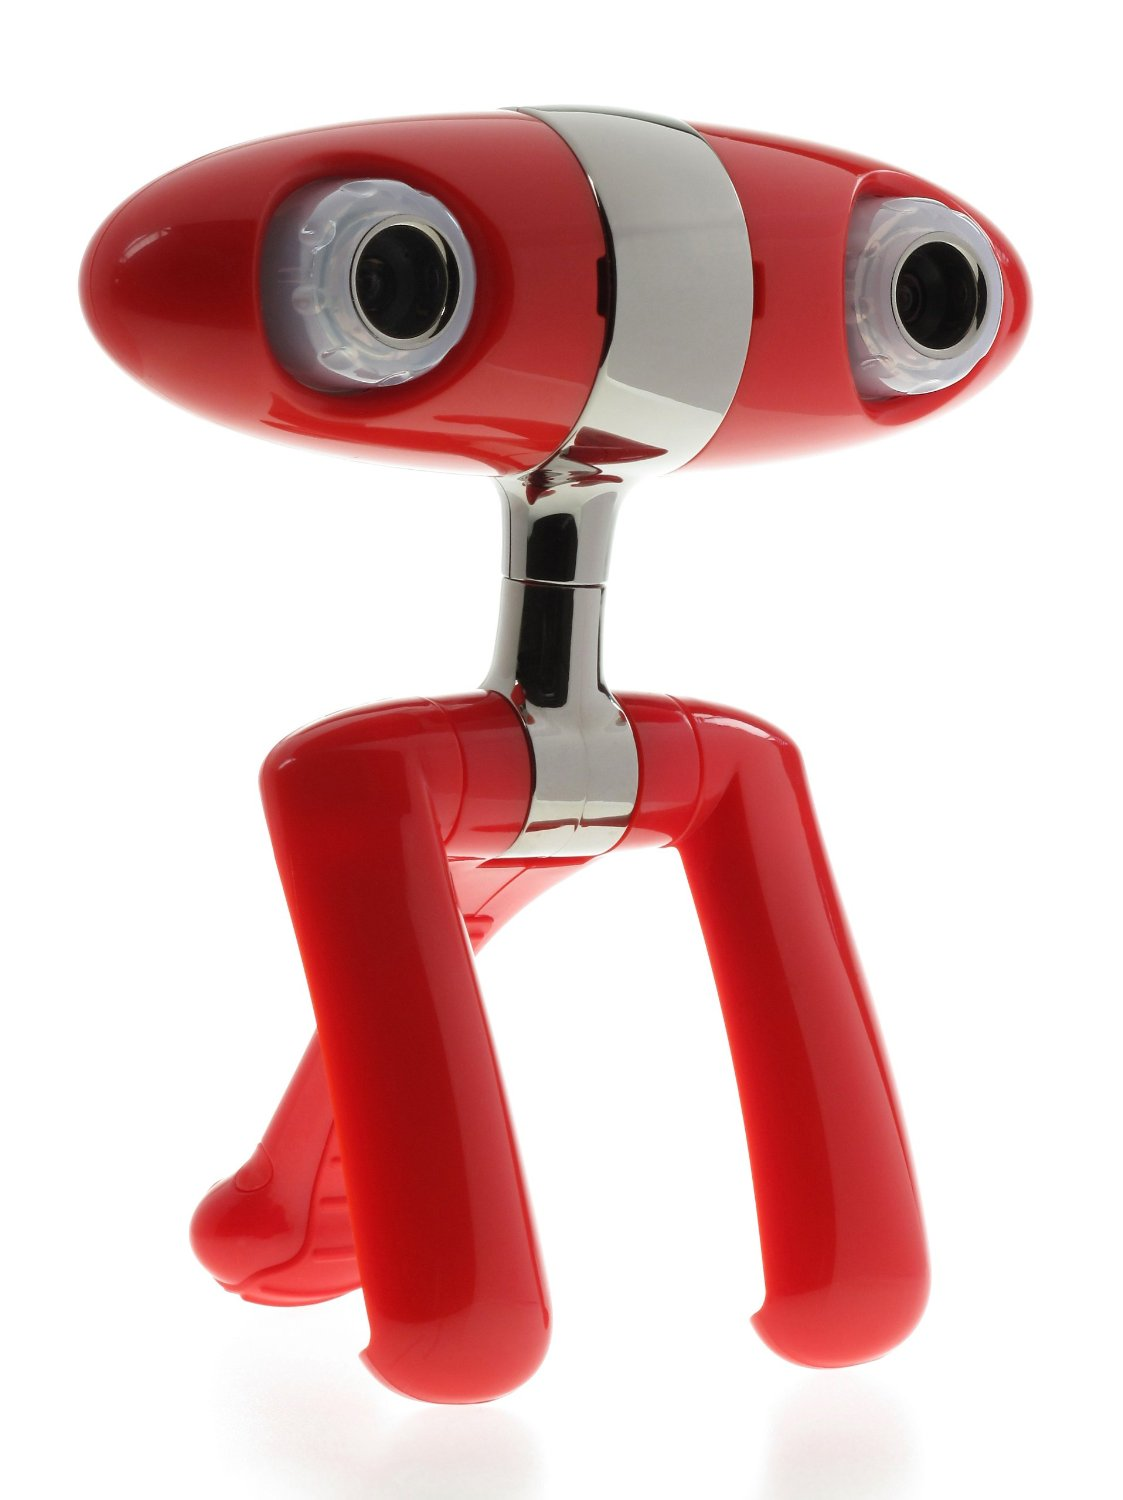
\includegraphics[scale=0.10]{./Resources/minoru.jpg}
	\caption{3D Webcam Minoru}
	\label{minoru}
\end{figure}

\begin{table}[]
\centering
\caption{Especificações - 3D Webcam Minoru}
\label{minoru_tab}
\begin{tabular}{|c|c|}
\hline
\textbf{Sensor de Imagem}      & VGA CMOS Sensor  	\\	\hline
\textbf{Resolução Máxima}      & $800x600$        	\\	\hline
\textbf{Tamanho Linha de Base} & 6 cm             	\\	\hline
\textbf{Taxa de Captura}       & 30 fps             	\\	\hline
\textbf{Distância Focal}       & 10 cm até $\infty$	\\	\hline
\textbf{Campo de Visão}        & $42\degree$		\\	\hline
\textbf{Peso}		       & 249.48 g		\\	\hline
\end{tabular}
\end{table}

Atualmente, a câmera utilizada é a digital 3D W3 fabricada pela Fujifilm (veja figura \ref{fujiW3}). A primeira câmera foi substituída, pois o controlador USB não permitia que a webcam realizasse \textit{streaming} na máxima resolução. Deste modo, optou-se por uma com maior resolução e que apresentasse lentes com baixa distorção. Entretanto, essa não apresenta \textit{streaming} via USB, assim é necessário que os vídeos sejam processados \textit{offline}. Visto que o projeto preocupa-se principalmente na identificação de obstáculos, isso não oferece nenhuma desvantagem para o desenvolvimento do trabalho. Todavia, para uma aplicação real, a câmera instalada no veículo deve apresentar esse aspecto. A tabela \ref{fujiW3_tab} apresenta as especificações da câmera em questão.

\begin{table}[]
\centering
\caption{Especificações - Câmera Digital Fujifilm FinePix Real 3D W3}
\label{fujiW3_tab}
\begin{tabular}{|c|c|}
\hline
\textbf{Sensor de Imagem}      & 10 MP CCD Sensor  	\\	\hline
\textbf{Resolução Máxima}      & $1280x720$        	\\	\hline
\textbf{Tamanho Linha de Base} & 7.5 cm             	\\	\hline
\textbf{Taxa de Captura}      & 24 - 30 fps          	\\	\hline
\textbf{Distância Focal}       & 60 cm até $\infty$	\\	\hline
\textbf{Peso}       		      & 250g		\\	\hline
\end{tabular}
\end{table}

\begin{figure}[H]
	\centering
	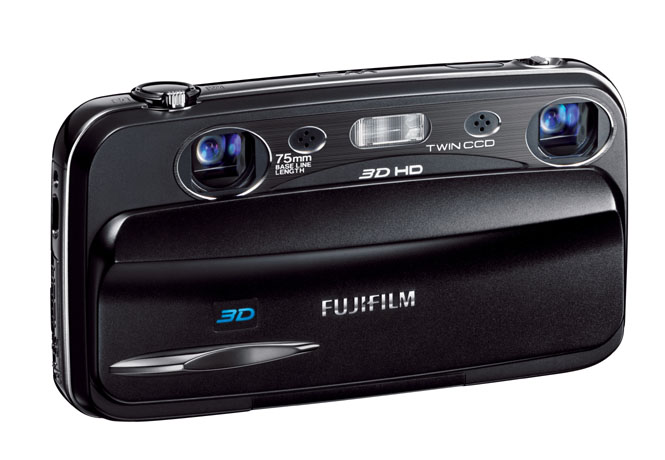
\includegraphics[scale=0.35]{./Resources/fujiW3.jpg}
	\caption{Câmera Digital Fujifilm FinePix Real 3D W3}
	\label{fujiW3}
\end{figure}


%-----------------------------------------------------------------------------------------------------------------------------------------------------------------------------------------------
\subsection{Unidades de Processamento}

Visto que este trabalho busca a implementação dos métodos estéreo em quadricópteros, tem-se como objetivo sua implementação para Linux embarcado (\textit{Embedded Linux}). Em seguida, estão apresentadas as plataformas que foram utilizadas para este propósito.


%-----------------------------------------------------------------------------------------------------------------------------------------------------------------------------------------------
\subsubsection{BeagleBone Black}

A primeira a ser utilizada e estudada é a plataforma aberta BeagleBone Black (BBB), ilustrada pela figura \ref{bbb}. Esta plataforma foi escolhida devido ao seu tamanho reduzido, podendo ser facilmente embarcada, isto é, é possível adaptá-la mecanicamente ao veículo. Com relação ao seu poder de processamento, ela apresenta um processador ARM Cortex-A8 operando à 1 GHz. A tabela \ref{bbb_tab} apresenta as especificações da plataforma.

\begin{table}[]
\centering
\caption{Especificações - BeagleBone Black}
\label{bbb_tab}
\begin{tabular}{|c|c|}
\hline
\textbf{Processador}           & 1GHz TI Sitara AM3359 ARM Cortex-A8			\\	\hline
\textbf{RAM}                   & 512 MB DDR3L @ 400 MHz					\\	\hline
\textbf{Armanezamento}         & 2 GB on-board eMMC, MicroSD				\\	\hline
\textbf{Sistemas Operacionais} & Angstrom (Default), Ubuntu, Android, dentre outros...	\\	\hline
\textbf{Consumo de energia}    & 210-460 mA @ 5V					\\	\hline
\textbf{Pinos de GPIO}         & 65/92 pinos						\\	\hline
\textbf{Periféricos}           & 1 USB Host, 1 Mini-USB Client, 1 10/100 Mbps Ethernet  \\	\hline                              
\end{tabular}
\end{table}

\begin{figure}[H]
	\centering
	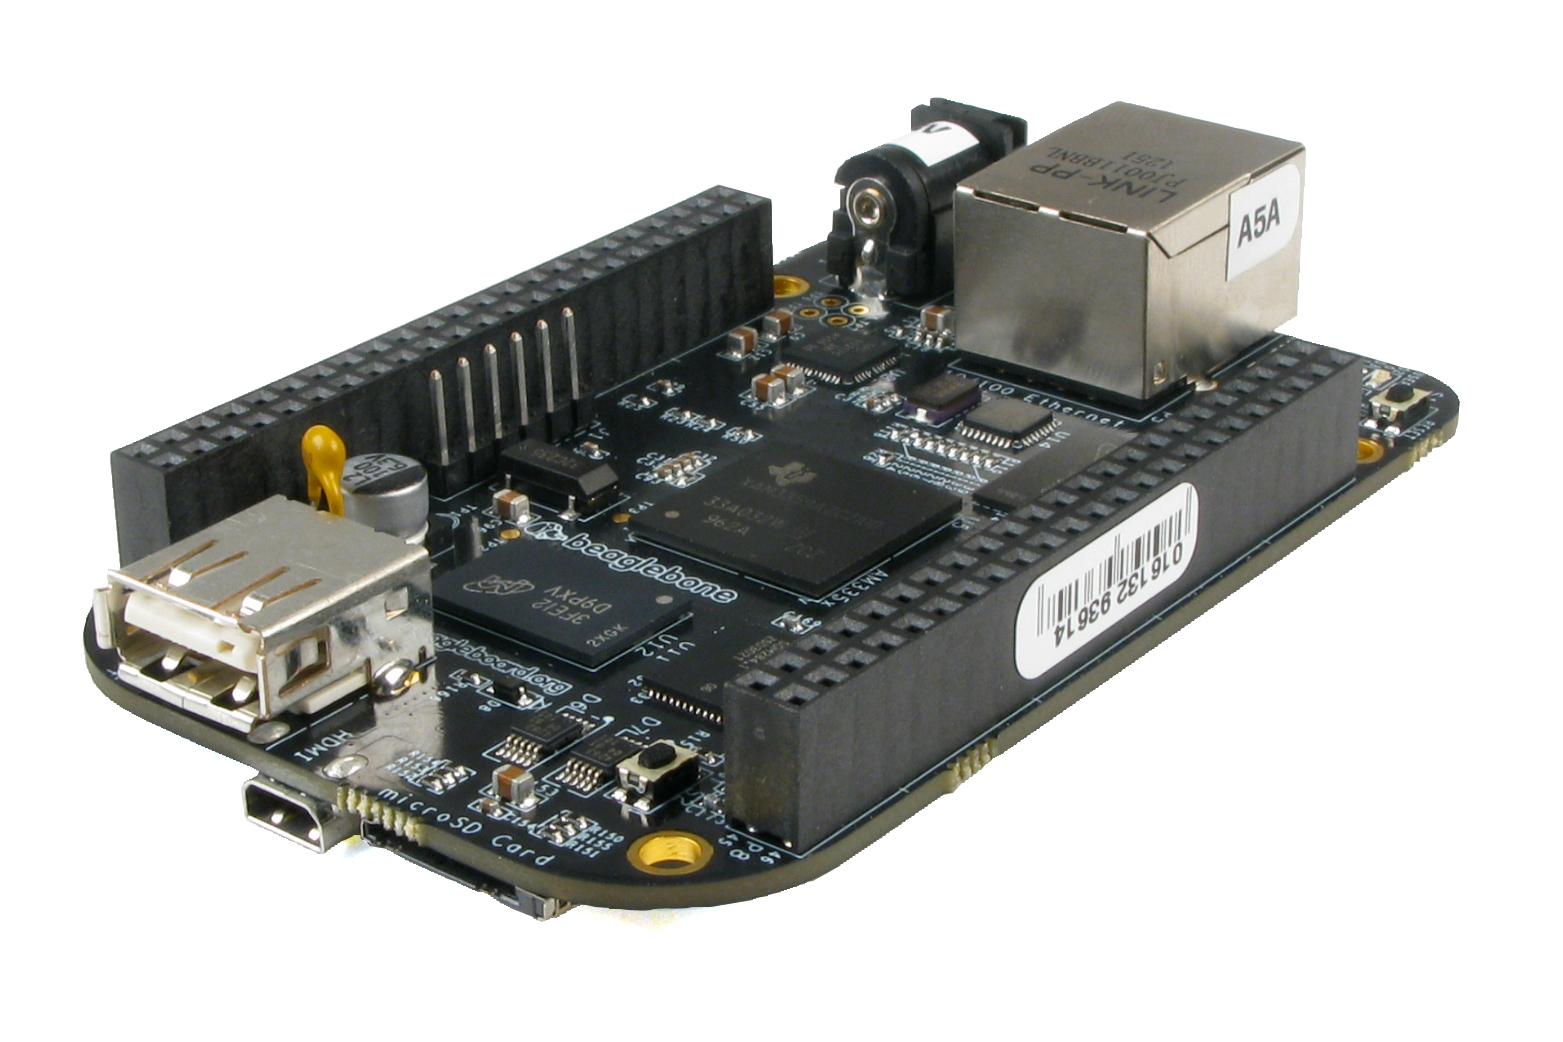
\includegraphics[scale=0.10]{./Resources/bbb.jpg}
	\caption{Plataforma de Desenvolvimento - BeagleBone Black}
	\label{bbb}
\end{figure}


%-----------------------------------------------------------------------------------------------------------------------------------------------------------------------------------------------
\subsubsection{Jetson TK1}

A segunda a ser utilizada e estudada é a plataforma Jetson TK1 produzida pela NVIDIA, figura \ref{jetson_tk1}. Essa plataforma conta com um processador de 32-bits Tegra K1 baseado na tecnologia ARM Cortex-A15. O motivo pelo qual esta plataforma foi escolhida é devido ao seu poder de processamento gráfico, visto que apresenta 192 núcleos gráficos, sendo assim adequada para aplicações envolvendo processamento de imagens. A tabela \ref{jetson_tk1_tab} apresenta as especificações da plataforma. Outro fator interessante desta plataforma é que ela oferece suporte à tecnologia CUDA, a qual será discutida mais adiante.

\begin{table}[]
\centering
\caption{Especificações - Jetson TK1}
\label{jetson_tk1_tab}
\begin{tabular}{|c|c|}
\hline
\textbf{Processador}           & NVIDIA 2.32GHz ARM quad-core Cortex-A15              \\	\hline
\textbf{Processador Gráfico}   & NVIDIA Kepler "GK20a" GPU  with 192 SM3.2 CUDA cores \\	\hline
\textbf{DRAM}                  & 2GB DDR3L 933MHz EMC x16 using 64-bit data width     \\	\hline
\textbf{Armanezamento}         & 16GB fast eMMC 4.51 (routed to SDMMC4)               \\	\hline
\textbf{Sistemas Operacionais} & Platforma 64-bit Linux Ubuntu 14.04                  \\	\hline
\textbf{Consumo de energia}    & 0.6W to 3W @ 12 V                                    \\	\hline
\textbf{Pinos de GPIO}         & 7 x GPIO pins (1.8V)                                 \\	\hline
\textbf{Periféricos}           & USB, mini-PCIe, SATA, SD-card, HDMI, audio           \\	\hline
\end{tabular}
\end{table}

\begin{figure}[H]
	\centering
	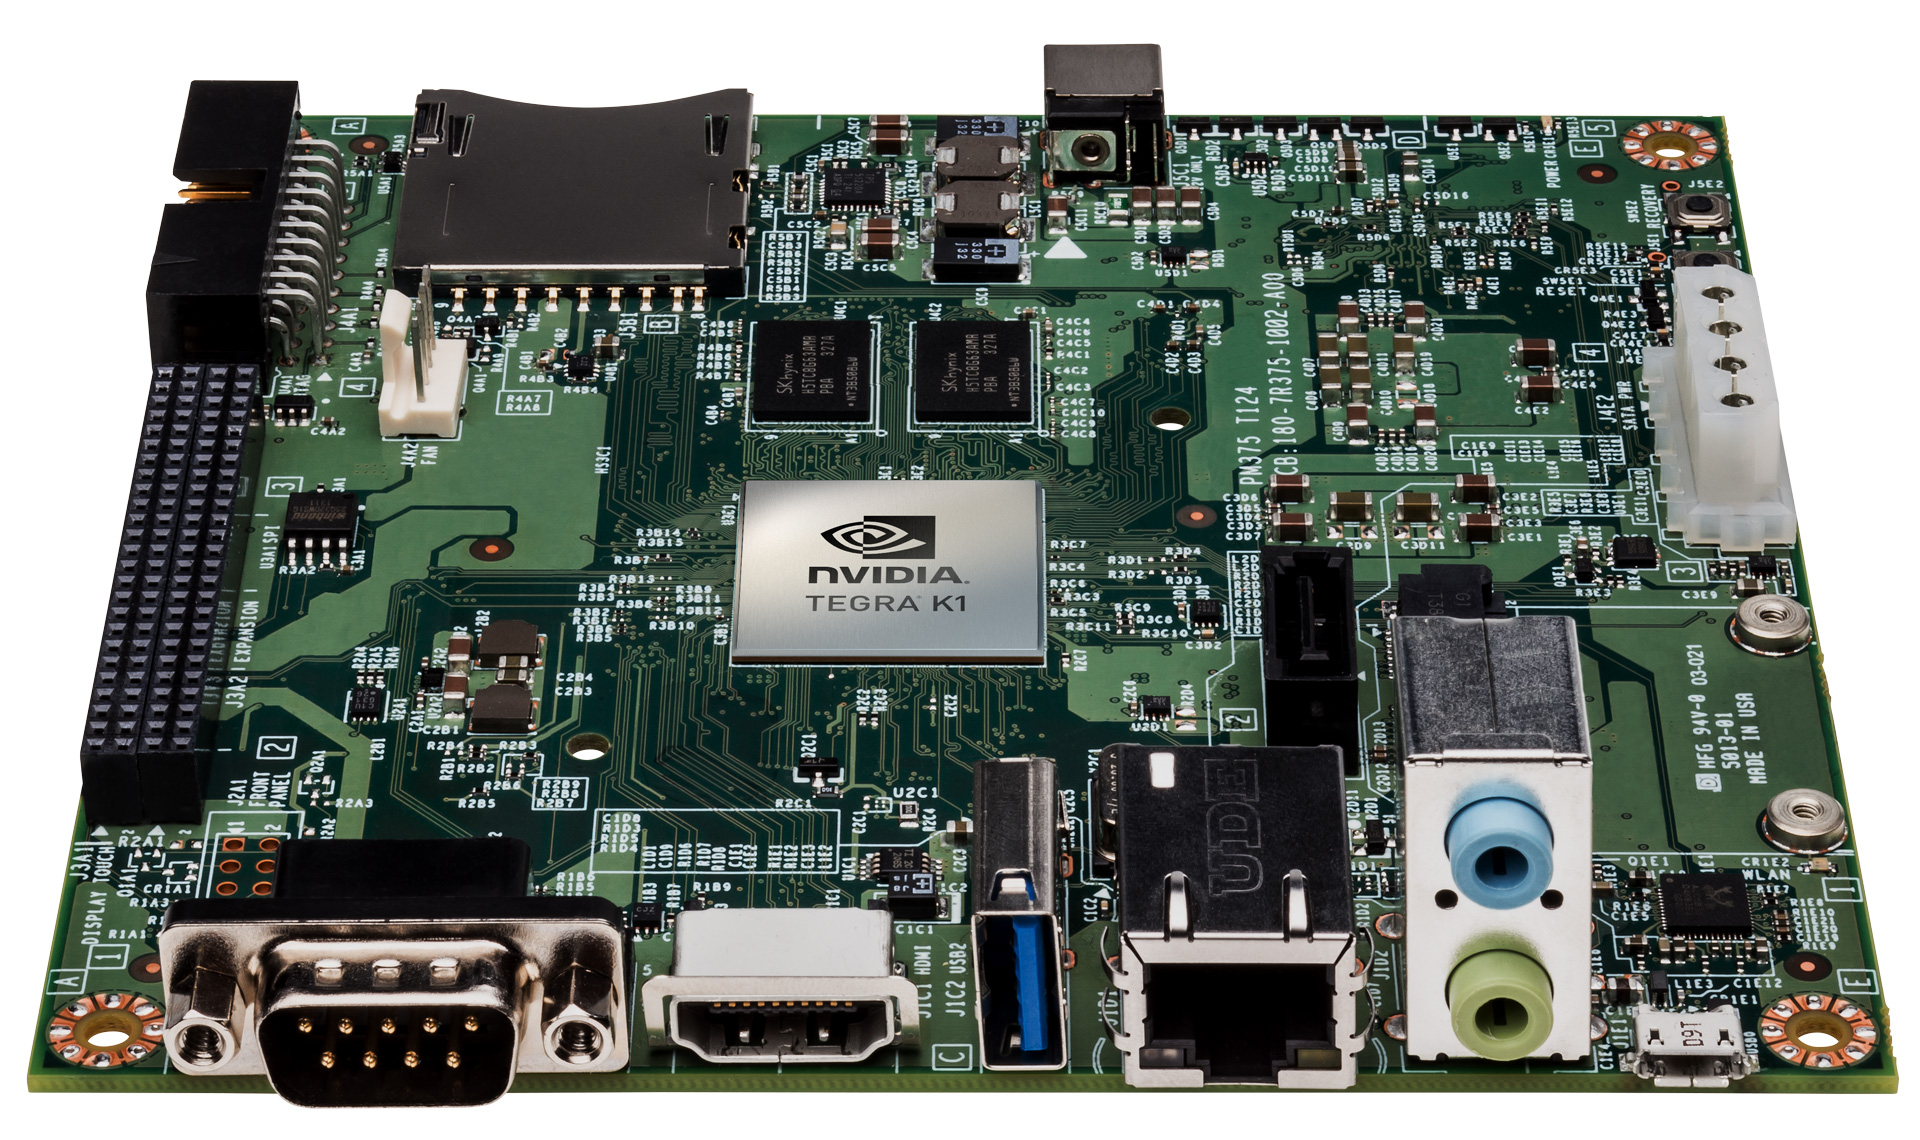
\includegraphics[scale=0.10]{./Resources/jetson_tk1.jpg}
	\caption{Plataforma de Desenvolvimento - Jetson TK1}
	\label{jetson_tk1}
\end{figure}


%-----------------------------------------------------------------------------------------------------------------------------------------------------------------------------------------------
\subsubsection{Notebook Asus Q550LF}

A terceira plataforma utilizada é um \textit{Notebook} Asus Q550LF, ela foi utilizada para o desenvolvimento de todos os programas contidos neste trabalho e para estudo de desempenho comparativo com as plataformas embarcadas. A interface desenvolvida, \textit{StereoVisionGUI}, foi desenvolvida para ser executada nesta máquina e em computadores com arquitetura x86 e x64. As espeficações desta plataforma estão apresentadas pela tabela \ref{asusQ550LF}.

\begin{table}[]
\centering
\caption{Especificações - Asus Q550LF}
\label{asusQ550LF}
\begin{tabular}{|c|c|}
\hline
\multicolumn{2}{|c|}{\textbf{Especificações CPU}}                                                   \\ \hline
\textbf{CPU}             & Intel Core i7 (4th Gen) 4500U / 1.8~3.0 GHz                              \\ \hline
\textbf{Number of Cores} & Dual-Core                                                                \\ \hline
\textbf{Memory}          & DDR3 SDRAM 8 GB                                                          \\ \hline
\multicolumn{2}{|c|}{\textbf{Espeficações de GPU}}                                                  \\ \hline
\textbf{Chipset}         & NVIDIA                                                                   \\ \hline
\textbf{Architecture}    & Kepler                                                                   \\ \hline
\textbf{GPU}             & GK107 384 @ 837 MHz                                                      \\ \hline
\textbf{Memory}          & DDR3 - 2048 MB - 128 Bit @ 1800 MHz                                      \\ \hline
\textbf{CUDA Cores}      & 384 Cores                                                                \\ \hline
\textbf{Features}        & Optimus, GPU Boost 2.0, PhysX, Verde Drivers, CUDA, 3D Vision, 3DTV Play \\ \hline
\end{tabular}
\end{table}


%-----------------------------------------------------------------------------------------------------------------------------------------------------------------------------------------------
\subsection{Equipamentos auxiliares}

Nesta seção, estão apresentados os equipamentos auxiliares para o desenvolvimento do trabalho. 

Os métodos para a identificação de correspondências entre as câmeras requerem que a imagem estejam calibradas e retificadas. Por conta disso, utiliza-se o padrão de calibração de dimensão 7x10, apresentado na figura \ref{calibration_pattern}, para este propósito. Deste modo, é possível caracterizar as distorções das lentes, parâmetros intrínsecos, e o posicionamento de uma das câmeras com relação a outra, parâmetros extrínsecos.  

\begin{figure}[H]
	\centering
	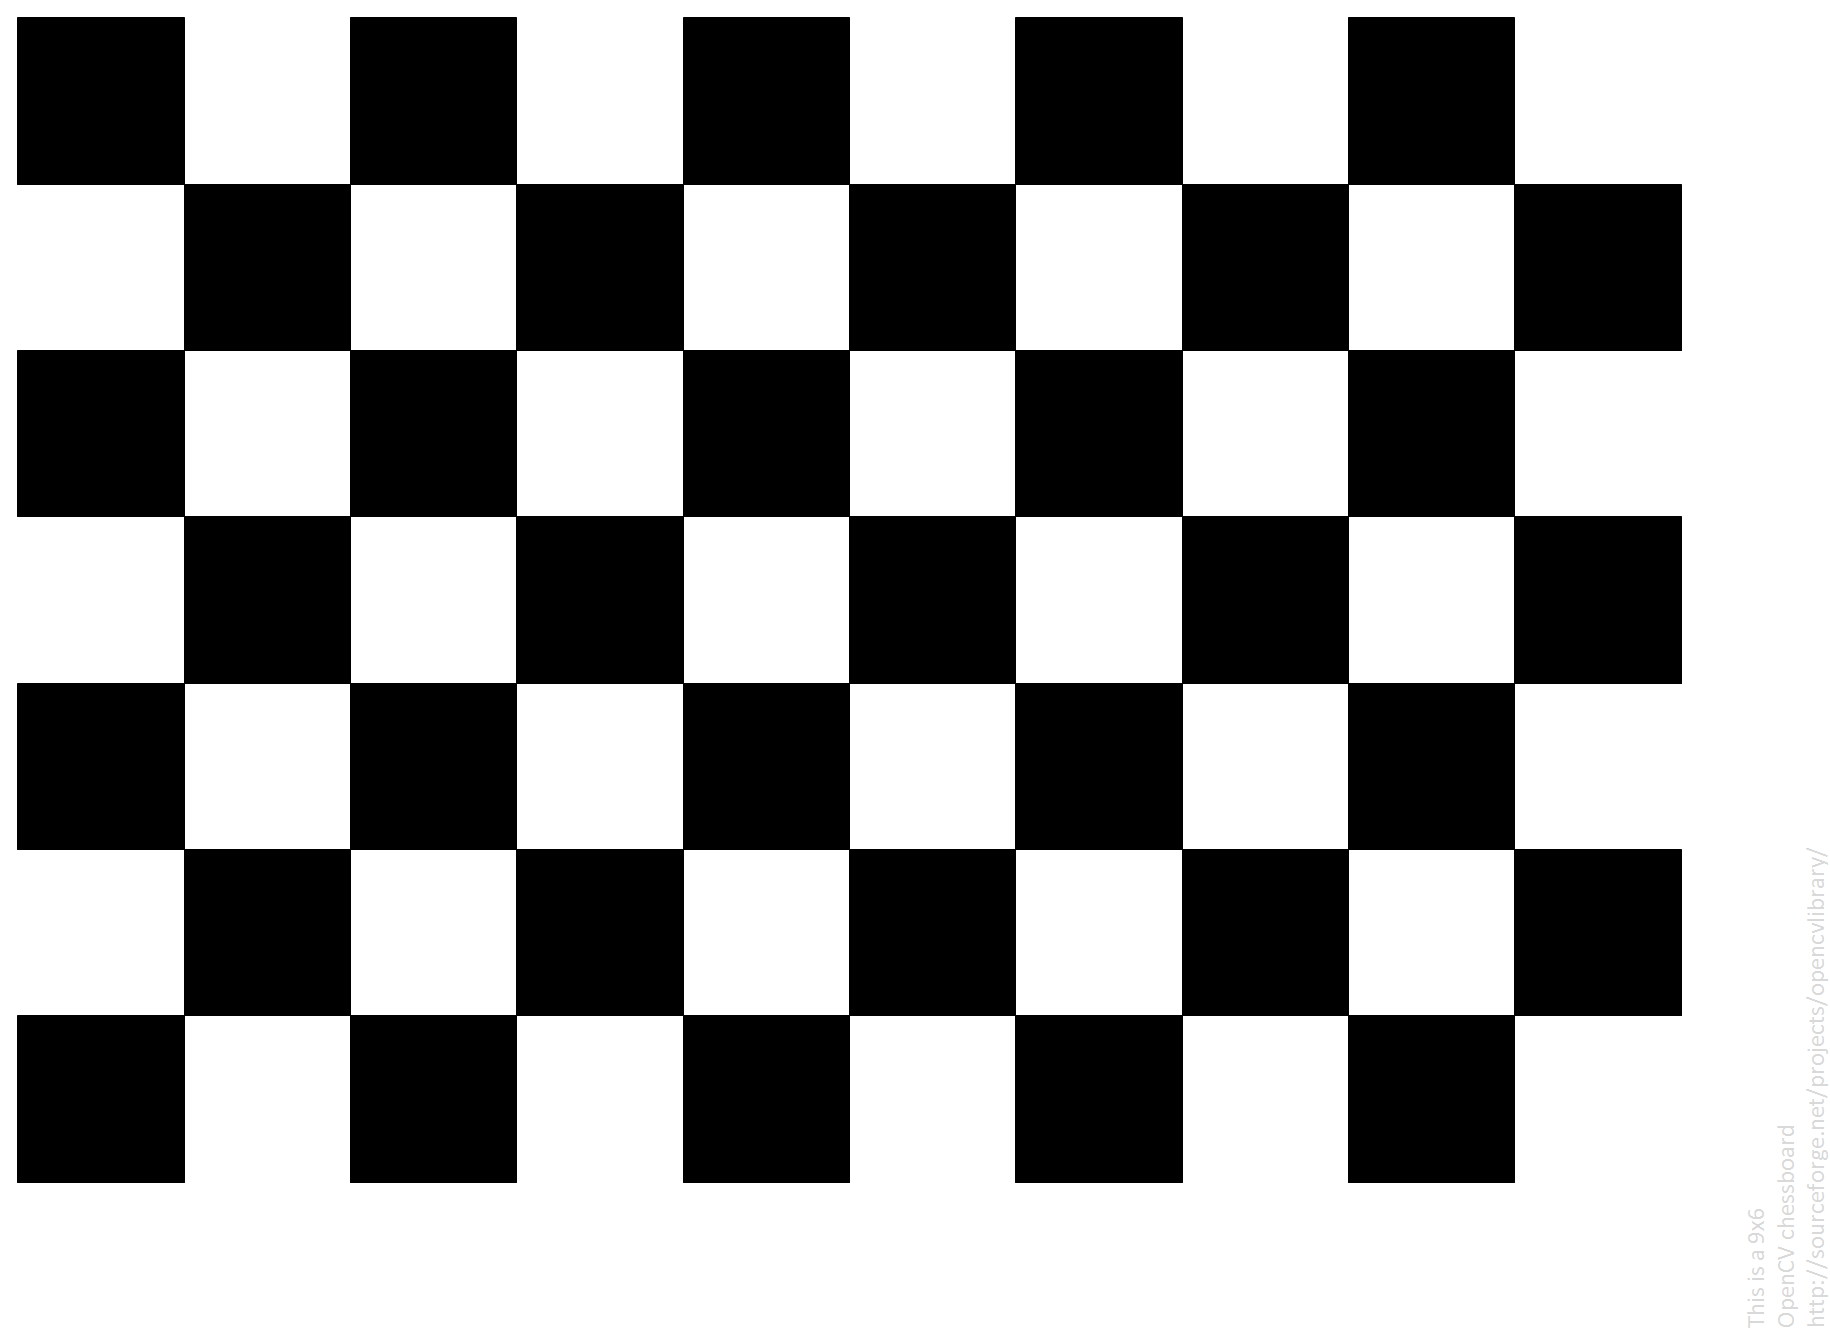
\includegraphics[scale=0.10]{./Resources/calibration_pattern.png}
	\caption{Padrão de Calibração}
	\label{calibration_pattern}
\end{figure}

A motivação deste trabalho é a sua utilização em veículos aéreos. Por conta disso, é indispensável que se tenha algum desses veículos. O trabalho conta com a utilização de um quadricóptero produzido pela 3DR, porém este apresenta modificações visando o seu desenvolvimento para navegação autônoma. Deste modo, tem-se a adição de \textit{propellers guards}, objetivando o aumento da segurança do veículo e das pessoas que o operam. Além disso, o \textit{drone} conta com suportes para a câmera estéreo e para a plataforma embarcada. Como pode ser observado na figura \ref{quad_camera_support}, todas as peças foram produzidas utilizando impressora 3D.

\begin{figure}[H]
	\centering
	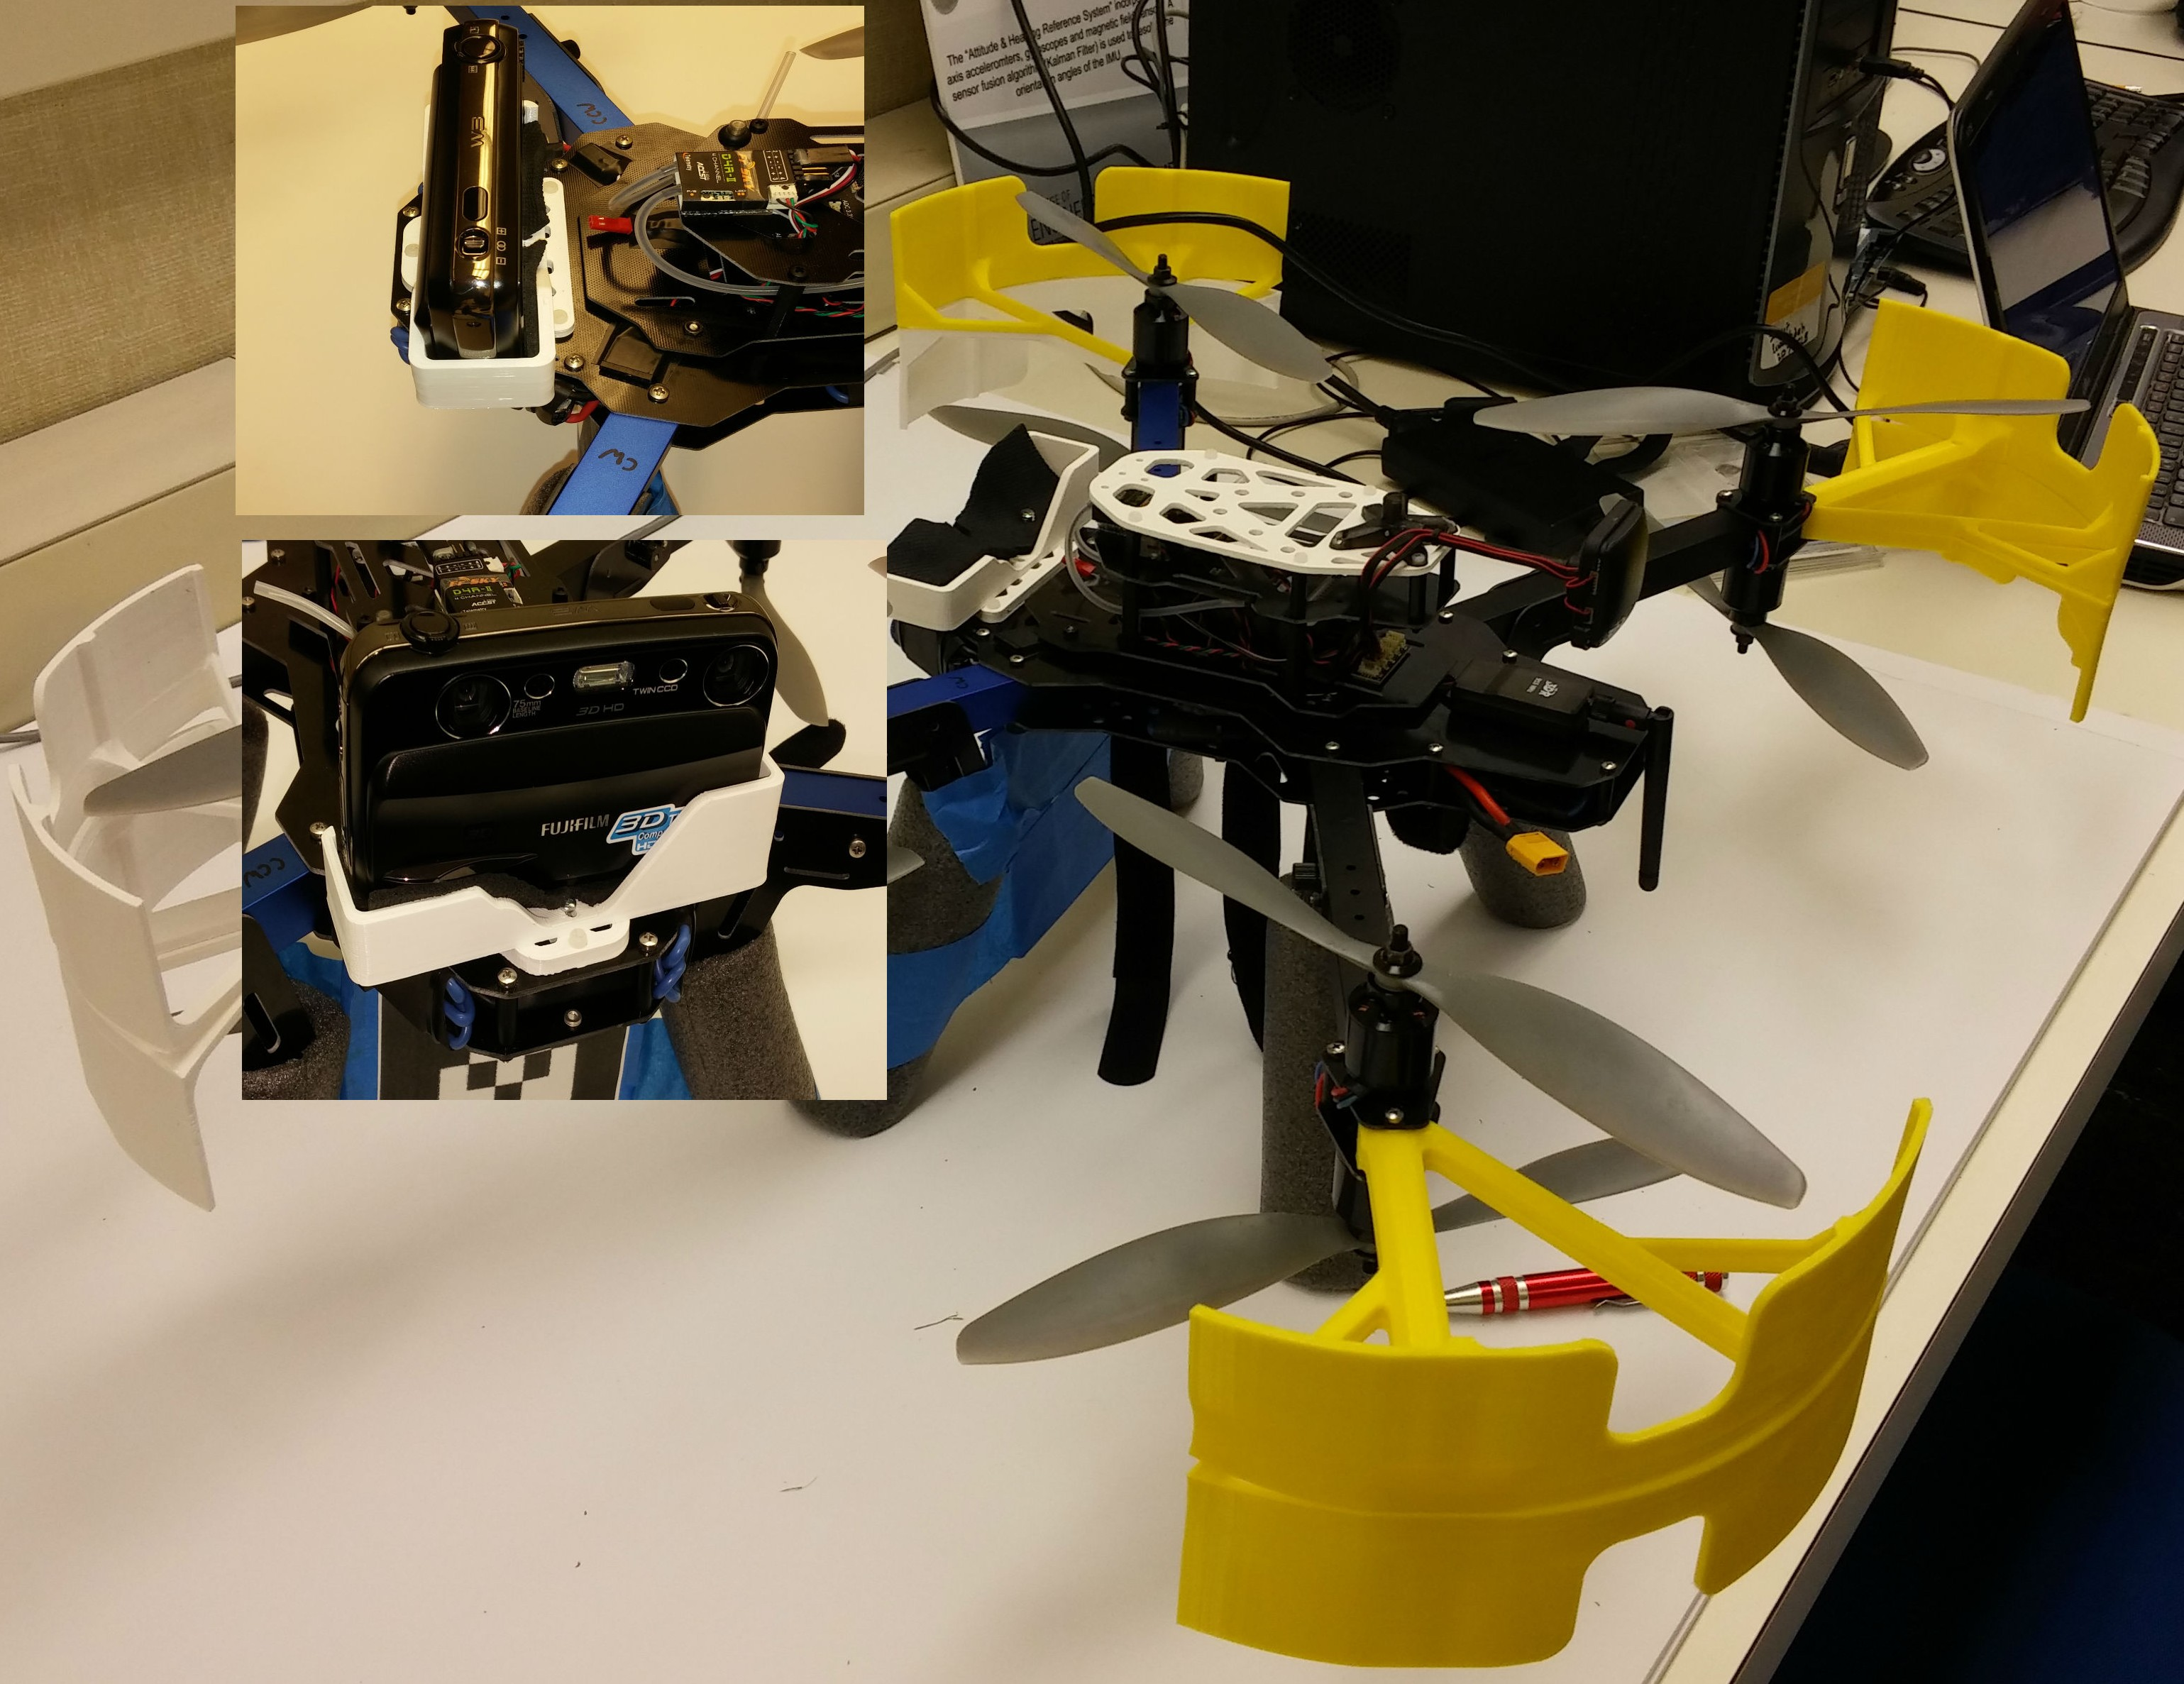
\includegraphics[scale=0.10]{./Resources/quad_camera_support.jpg}
	\caption{Quadricóptero 3DR X8 com suporte para a Câmera 3D}
	\label{quad_camera_support}
\end{figure}


%-----------------------------------------------------------------------------------------------------------------------------------------------------------------------------------------------
\section{Métodos}

Nesta seção, serão apresentados os cenários e os procedimentos utilizados na implementação dos métodos estéreo apresentados.


%-----------------------------------------------------------------------------------------------------------------------------------------------------------------------------------------------
\subsection{Cenários}

O pós-processamento do mapa de disparidades foi voltado para a identificação e detecção de obstáculos. Deste modo, os seguintes cenários propõe uma série de adversidades, as quais o algoritmo implementado tenta contorná-las. Propôs-se que ele deve ser flexível à variações na luminosidade, capaz de detectar obstáculos estáticos e móveis, e ser imune à vibrações. Deste modo, dois cenários em ambiente confinado e um em ambiente aberto foram analisados. Deseja-se a navegação autônoma ocorra até mesmo em casos que o sinal do Sistema de Posicionamento Global (GPS) seja perdido, por conta disso escolheu-se a utilização dos ambientes confinados. O ambiente externo foi escolhido devido a quantidade de fatores externos que poderiam atrapalhar a detecção de obstáculos. O tratamento destes percalços tornam o programa mais robusto.


%-----------------------------------------------------------------------------------------------------------------------------------------------------------------------------------------------
\subsubsection{Cenário 1}

O cenário da figura \ref{thumb_video10_l} foi utilizado para estudo das condições de ambiente externo, o qual está sujeito grandes variações de luminosidade e um número menor de movimentos, o que permite uma análise de alcances maiores. O principal  obstáculo deste cenário é uma árvore. 


%-----------------------------------------------------------------------------------------------------------------------------------------------------------------------------------------------
\subsubsection{Cenário 2}

O cenário da figura \ref{thumb_video12_l} foi utilizado para estudo das condições de ambiente interno, o qual também apresenta certa variação de luminosidade, porém apresenta um número maior de movimentos, permitindo uma análise de objetos estáticos à curta e média distância. Os principais obstáculos deste cenário são uma mesa, uma cadeira e duas estantes.


%-----------------------------------------------------------------------------------------------------------------------------------------------------------------------------------------------
\subsubsection{Cenário 3}

O cenário da figura \ref{thumb_video15} foi utilizado para estudo das condições de ambiente interno, o qual também apresenta certa variação de luminosidade, apresenta um número muito maior de movimentos e permite a análise de objetos móveis à curto e médio alcance. Os principais obstáculos deste cenário  é uma bancada e um outro quadricóptero no campo de visão do veículo pilotado.


%-----------------------------------------------------------------------------------------------------------------------------------------------------------------------------------------------
% Figuras
\begin{figure}[H]
	\centering
	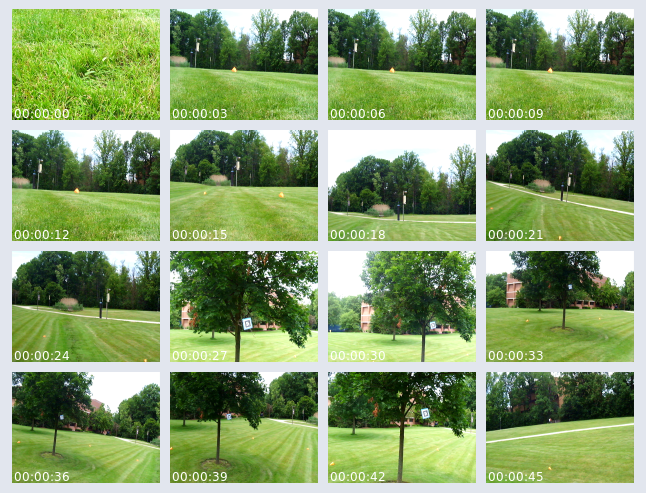
\includegraphics[scale=0.55]{./Resources/thumbs/thumb_video10_l.png}
	\caption{Cenário 1 - Ambiente Externo - Árvore}
	\label{thumb_video10_l}
\end{figure}

\begin{figure}[H]
	\centering
	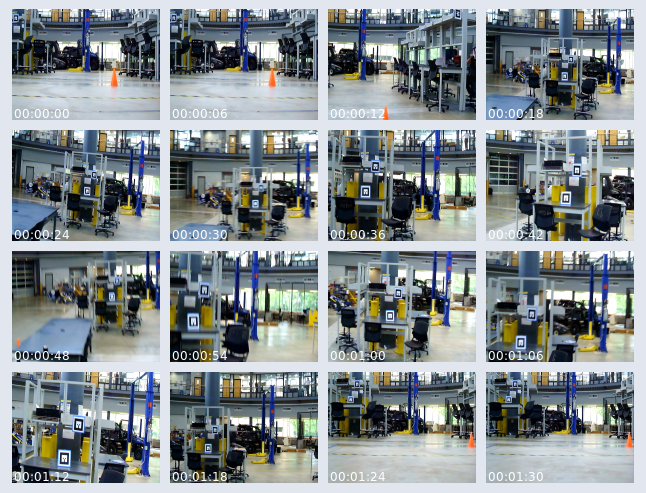
\includegraphics[scale=0.55]{./Resources/thumbs/thumb_video12_l.png}
	\caption{Cenário 2 - Ambiente Interno - Mesa/Cadeira/Estantes}
	\label{thumb_video12_l}
\end{figure}

\begin{figure}[H]
	\centering
	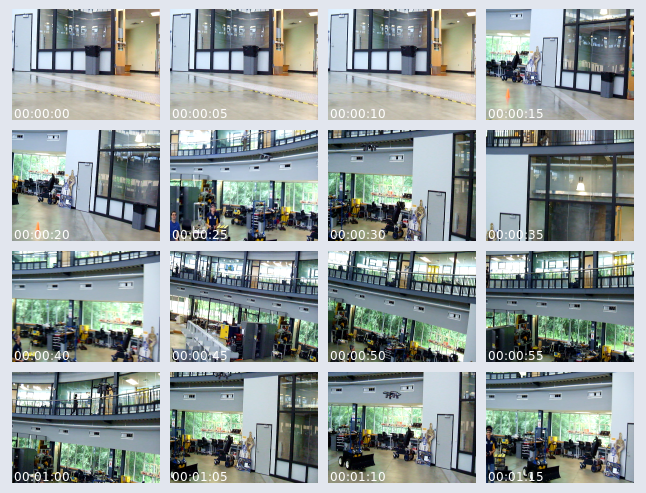
\includegraphics[scale=0.55]{./Resources/thumbs/thumb_video15.png}
	\caption{Cenário 3 - Bancada/Quadricóptero}
	\label{thumb_video15}
\end{figure}


%-----------------------------------------------------------------------------------------------------------------------------------------------------------------------------------------------
\subsection{Processamento de Imagem}

Nessa seção será apresentado o processamento de imagens utilizado para a identificação de obstáculos. Como pode ser visto na figura \ref{stereo_processor_steps}, todo o processo conta com seis etapas.

\textbf{Câmeras:} O primeiro passo do processo é a captura das imagens da câmera estéreo. Idealmente, as imagens deve ser capturadas ao mesmo instante e as lentes não apresentarem distorções.   

\textbf{Calibração e Retificação:} Na prática, as lentes apresentam distorção. Com base nos parâmetros obtidos após a calibração das câmeras é possível retificá-las. 

\textbf{Correspondência Estéreo:} Aplica-se os métodos para encontrar as correspondências entre as duas câmeras, gerando assim o mapa de disparidades.

\textbf{Pré-filtragem:} Este passo, pode ser aplicado tanto nas imagens retificados ou no mapa de disparidades. Atualmente, aplica-se a operação morfológica de abertura e um filtro de Mediana sobre o mapa de disparidades. 

\textbf{Limiarização por Distância:} Visto que a disparidade apresenta uma relação com a distância, aplica-se uma operação de limiarização. Deste modo, apenas os obstáculos a uma certa distância são segmentados.

\textbf{Identificação de Obstáculos:} Após o passo anterior, o objeto é identificado e sua posição é rastreada. Essa informação pode ser utilizada pelo sistema de controle da aeronave para manter distância do obstáculo identificado.

\begin{figure}[H]
	\centering
	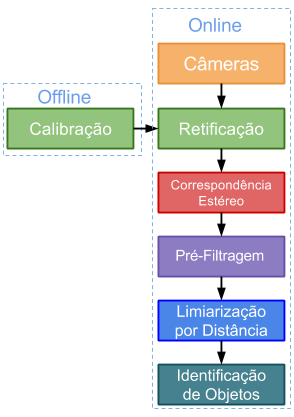
\includegraphics[scale=0.50]{./Resources/stereo_processor_steps2.png}
	\caption{Etapas do Processamento de Imagens}
	\label{stereo_processor_steps}
\end{figure}


%-----------------------------------------------------------------------------------------------------------------------------------------------------------------------------------------------
\subsection{Aceleração em Hardware - \textit{Hardware Acceleration}}
\subsubsection{CUDA}

Neste trabalho, utilizou-se diferentes versões desta plataforma para o desenvolvimento para \textit{Desktop} e Jetson TK1. Neste contexto, essas versões não oferencem nenhuma alteração visível, visto que não foi desenvolvido nenhum tipo de rotina espeficamente para execução em GPU. Na verdade, utilizou-se as funções disponíveis na biblioteca OpenCV, as quais opcionalmente podem ser executadas pela CPU ou GPU. A tabela \ref{cudaopencv} informa as versões do pacote de ferramentas da plataforma CUDA e da biblioteca OpenCV utilizadas. 

\begin{table}[]
\centering
\caption{Versões utilizadas de CUDA e OpenCV}
\label{cudaopencv}
\begin{tabular}{cccll}
                     & \textbf{CUDA ToolKit}	     & \textbf{OpenCV} 	       &  &  \\
\textbf{Desktop}     & 7.5                           & 3.0.0                   &  &  \\
\textbf{Jetson TK1}  & 6.5                           & 2.4.12                  &  &  \\
\multicolumn{1}{l}{} & \multicolumn{1}{l}{}          & \multicolumn{1}{l}{}    &  & 
\end{tabular}
\end{table}

%-----------------------------------------------------------------------------------------------------------------------------------------------------------------------------------------------
% TODO: NEON
\subsubsection{NEON}


%-----------------------------------------------------------------------------------------------------------------------------------------------------------------------------------------------
\subsection{Jetson TK1 - Configuração da Plataforma}

A execução das rotinas de visão estéreo com aceleração via GPU requisitam que a plataforma de desenvolvimento esteja corretamente configurada. Abaixo, encontra-se o tutorial para configurá-la para a operação desejada, isto é,basicamente, configurá-la para o correto funcionamento da CUDA e do OpenCV2. 

\begin{enumerate}
  \item Baixando o JetPack L4T
    \begin{enumerate}
      \item Clique \href{http://docs.nvidia.com/jetpack-l4t/index.html#developertools/mobile/jetpack/jetpack_l4t/2.1/jetpack_l4t_install.htm}{aqui} para ir ser redirecionado para a página do pacote de desenvolvimento Jetpack L4T. Caso o link esteja quebrado, vá até o página da NVIDIA e procure pelo localização correta do pacote.  

      \item Na máquina \textit{Host} rodando Ubuntu, crie um novo diretório para armazenar os pacotes de instalação utilizando as seguintes linhas de comando.
      \begin{lstlisting}[basicstyle=\tiny]
	$ ubuntu@ubuntu:~$ cd /home/<user>
	$ ubuntu@ubuntu:~/home/<user>$ mkdir flash
	$ ubuntu@ubuntu:~/home/<user>$ cd flash
	$ ubuntu@ubuntu:~/home/<user>/flash$ 
      \end{lstlisting}
      Uma ação importante que merece destaque é baixar o arquivo JetPack-\${VERSION}.run dentro do diretório criado (o caminho NÃO DEVE conter espaços).
      
      \item Dê permissão de execução para o arquivo baixado. 
      \begin{lstlisting}[basicstyle=\tiny]
	$ ubuntu@ubuntu:~/home/<user>/flash$ chmod +x JetPack-${VERSION}.run
	$ ubuntu@ubuntu:~/home/<user>/flash$ ./JetPack-${VERSION}.run
      \end{lstlisting}
      
      
    \end{enumerate}
  \item Instalando o JetPack L4T
  
    Sigua as instruções no manual de usuário do kit de desenvolvimento da Jetson TK1
    \begin{enumerate}
      \item Baixe o guia de instruções no seguinte link e clique na aba "\textit{Install Guide}". Link: \url{https://developer.nvidia.com/embedded/jetpack}
      \item Sigua as instruções do instalador do Jetpack L4T.
     
      Uma informação que merece destaque é que o computador \textit{Host} e o dispositivo alvo (Jetson TK1) DEVEM estar conectados à mesma rede. Isso pode ser feito conectando:
      \begin{enumerate}
	\item Máquina \textit{Host} e dispositivo alvo à mesma Intranet, no caso o dispositivo alvo tenha um endereço IP estático.
	\begin{lstlisting}[basicstyle=\tiny]
	    ----------------------------------------------------
	    Edite o /etc/network/interfaces:
	    ----------------------------------------------------    
	    auto lo
	    iface lo inet loopback
	    auto eth0
	    iface eth0 inet static
	    address 10.235.0.133
	    netmask 255.255.252.0
	    network 10.235.3.0
	    gateway 10.235.0.1
	    pre-up ifconfig eth0 hw ether 00:01:02:03:05:09
	    dns-nameservers  143.107.225.6 143.107.182.2 8.8.8.8
	 \end{lstlisting}
	 
	 \item Máquina \textit{Host} e dispositivo alvo ao mesmo roteador. Neste caso, o dispositivo alvo DEVE ser capaz de encontrar o endereço IP por protocolo DHCP.
	 \begin{lstlisting}[basicstyle=\tiny]
	    ----------------------------------------------------
	    Edite o /etc/network/interfaces:
	    ----------------------------------------------------    
	    auto eth0
	    allow-hotplug eth0
	    iface eth0 inet dhcp
	 \end{lstlisting}
      \end{enumerate}
     
   
     
    \end{enumerate}
  \item Instalando o OpenCV com Módulo GPU na Jetson TK1
  
  Primeiramente, deve-se baixar e instalar o pacote de ferramentas CUDA, uma vez que é necessário para OpenCV. Cabe ao usuário decidir se deseja-se utilizar a biblioteca pré-compilada ou compilar a biblioteca do código-fonte. A primeira opção é a mais recomendada, visto que a biblioteca pré-compilada é a OpenCV4Tegra, uma versão otimizada em CPU e GPU do OpenCV para a Jetson TK1. A segunda opção é recomendada caso deseja-se adicionar módulos que não estão presentes na versão OpenCV4Tetra \cite{eLinuxJetsonOpenCV}. 
  
\end{enumerate}